\documentclass[12pt]{article}
\setlength{\oddsidemargin}{0in}
\setlength{\evensidemargin}{0in}
\setlength{\textwidth}{6.5in}
\setlength{\parindent}{0in}
\setlength{\parskip}{\baselineskip}

\usepackage{amsmath,amsfonts,amssymb,graphicx,enumerate}


\begin{document}
\title{Algorithms Homework 3}

CSCI 3104 Spring 2017 \hfill Problem Set 3\\
Grant Baker (07/23)\\
Samuel Cuthbertson (06/16)\\
Connor Hudson (05/07)\\


\hrulefill

\begin{enumerate}

	\item \textit{Why do we analyze the average-case performance of a randomized algorithm and not its worst-case performance? Succinctly explain.}
	
	Because a randomized algorithm uses randomization to ensure that \textit{any} input, even a worst case input, will be processed in average case time. This can be proven probabilistically as well as with some clever 
recurrence relations, both of which are shown in the lecture notes.
	
	\newpage
	\item \textit{Solve the following recurrence relations using the recurrence tree method; include a diagram of your recurrence tree. If the recurrence relation describes the behavior of an algorithm you know, state its 
name.}
    
    \begin{enumerate}
    \item $T(n) = T\left(\lceil \frac{n}{2} \rceil\right) + 1$
    \[
    \begin{array}{ccccc|c}
    &&n&&&1\\ 
    &&\downarrow&&&\\
    &&\lceil\frac{n}{2}\rceil&&&1\\
    &&\downarrow&&&\\
    &&\lceil\frac{n}{4}\rceil&&&1\\
    &&\vdots&&&\vdots\\
    \end{array}
    \]
    We note that the ceiling operation does not change the height of the tree, since we can consider two cases for the size of the input $n$.
    
    In the case that $n=2k$, $k\in\mathbb{N}$, we can clearly see that 
    \[
    \left\lceil \frac{n}{2} \right\rceil = \left\lceil \frac{2k}{2} \right\rceil = k
    \]
    In the case that $n=2k-1$, $k\in\mathbb{N}$, we can also see that
    \[
    \left\lceil \frac{n}{2} \right\rceil = \left\lceil \frac{2k-1}{2} \right\rceil \leq \left\lceil \frac{2k}{2} \right\rceil = k
    \]
    
    Thus, $\boxed{T(n) = \Theta(\log_2 n)}$. This recurrence relation describes the running time for a binary search algorithm.\\
    
    \item $T(n) = 2T\left(\frac{n}{2}\right) + n$
    \[
    \begin{array}{ccccc|c}
    &&n&&&n\\
    &&\swarrow\searrow&&&\\
    &\frac{n}{2}&&\frac{n}{2}&&2\left(\frac{n}{2}\right)\\
    &\swarrow\searrow&&\swarrow\searrow&\\
    \frac{n}{4}&&\frac{n}{4}\hspace{12pt}\frac{n}{4}&&\frac{n}{4}&4\left(\frac{n}{4}\right)\\
    \vdots && \vdots\hspace{12pt}\vdots && \vdots & \vdots
    \end{array}
    \]
    We end up with a tree of height $\log_2 n$, where for level $i$ we require $\frac{2^i}{2^i}n=n$ computations. Therefore, our cost is the sum
    \[
    \sum_{i=0}^{\log_2 n}n = n\log_2 n = \boxed{\Theta(n\log_2 n)}
    \]
    This recurrence relation describes the running time for both Quicksort and Mergesort.
    
    \item $T(n) = 2T\left(\frac{n}{2}\right) + 1$
    \[
    \begin{array}{ccccc|c}
    &&n&&&1\\
    &&\swarrow\searrow&&&\\
    &\frac{n}{2}&&\frac{n}{2}&&2\left(1\right)\\
    &\swarrow\searrow&&\swarrow\searrow&\\
    \frac{n}{4}&&\frac{n}{4}\hspace{12pt}\frac{n}{4}&&\frac{n}{4}&4\left(1\right)\\
    \vdots && \vdots\hspace{12pt}\vdots && \vdots & \vdots
    \end{array}
    \]
    We end up with a tree of height $\log_2 n$, where for level $i$ we require $2^i=1$ computations. Therefore, our cost is the sum
    \[
    \sum_{i=0}^{\log_2 n}2^i = 2\cdot2^{\log_2 n} - 1 = 2n -1 = \boxed{\Theta(n)}
    \]
    This recurrence relation describes the runtime for a traversal of a binary tree.
    \end{enumerate}
    
    \newpage
    \item \textit{CLRS states that a red-black tree with n internal nodes has height at most $2 \log(n + 1)$. For a tree with $n = 10$, give a sequence of positive integers $\sigma = [\sigma_1,\sigma_2,...,\sigma_n]$ for $\sigma_i 
\in [1, 10]$, such that inserting that sequence into an empty red-black tree achieves the maximum height. Justify your claim.\footnote{Tip for ordering from Aaron Aaeng}}
    
    Note that the maximum height of a red-black tree is $2\log_2(n+1)$, where here $n$ is $10$. Therefore, we are looking for a tree of height $2\lg_2(11)=6$. Testing the base case of $[0,1,2,...,10]$, we found that the resultant 
tree is of height $6$, as shown below.\footnote{Visualization from \texttt{https://www.cs.usfca.edu/\~{}galles/visualization/RedBlack.html}}
    \begin{center}
        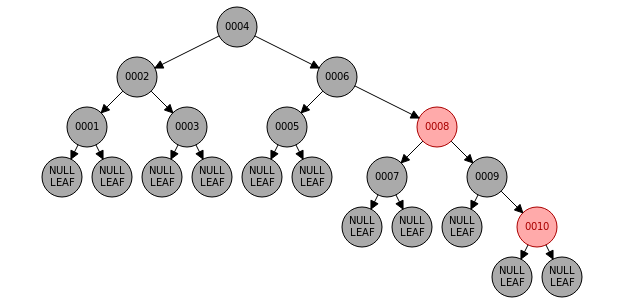
\includegraphics[width=.8\textwidth]{RedBlackMaxHeight.png}
    \end{center}
    \[
    \boxed{\sigma = [1,2,3,4,5,6,7,8,9,10]}
    \]
    This sequence of integers works because of the way trees handle inputs. If the input is ordered, then the root is the lowest element, each left child is null, and each right child is the next element. Red-black trees attempt to 
combat this by rebalancing the tree if needed. However, an ordered input still results in the tallest possible tree because we always add nodes to the right child of the rightmost child and require it to rebalance.\\
    
    Another justification for the correctness of this integer sequence is the note that for a red-black tree to be at a maximum height for a given size, all of the red nodes will be on the same path. In this case, the red nodes are 
all on the path $4\rightarrow6\rightarrow8\rightarrow9\rightarrow10$. Any red node that is not on this path would only serve to decrease the height of the tree.
    
    \newpage
    \item \textit{A peaked array has the property that the subarray $A[1..i]$ has the property that $A[j] < A[j + 1]$ for $1 \leq j < i$, and the subarray $A[i..n]$ has the property that $A[j] > A[j + 1]$ for $i \leq j < n$. Using 
her wand, McGonagall writes the following peaked array on the board $A = [7, 8, 10, 15, 16, 23, 19, 17, 4, 1]$, as an example.}
    \begin{enumerate}
        \item \textit{Write a recursive algorithm that takes asymptotically sub-linear time to find the maximum element of A. \footnote{Change of Binary Search condition from Luke Meszar}}
        
        \begin{verbatim}
findMaxPeaked(A) {
    return search(A,1,n) 
}

search(A,s,t) {
    if(s==t) return A[s]
    m = floor((s + t) / 2)
    if(A[m+1] < A[m])
    {
        if(A[m-1] < A[m]){
            return A[m]
        } else {
            return search(A,s,m-1)
        }
    } else {
        return search(A,m+1,t)
    }
}
        \end{verbatim}
        
    	\item \textit{Prove that your algorithm is correct. (Hint: prove that your algorithm's correctness follows from the correctness of another correct algorithm we already know.)}
    	
    	Let us note what our algorithm does: looks for a value which is greater that both of its immediate neighbors. Our loop invariant is then that the maximum value is somewhere in $A[l,...,r]$. \\
    	
    	At \textbf{initialization}, $s$ is necessarily the first element and $t$ is necessarily the last element because of how \textsf{search} is first called. On every \textbf{iteration}, assuming our invariant holds at the 
beginning of the call, we check to see if the current middle element, $A[m]$, fits our conditions for maximum. If it does, we simply return it. If not, we check to see if $A[m]>A[m+1]$, in which case our maximum is within 
$A[s,...,m]$. If, instead, $A[m]<A[m+1]$, we know that our maximum must necessarily be within $A[m,...,t]$ due to the nature of peaked arrays.\\
    	
    	Therefore, we can state that \textbf{termination} will occur as $s$ approaches $t$ with every call to \textsf{search}, which means that either we will encounter the maximum or our base case of $s=t$ will occur. \\
    
    	\item \textit{Now consider the multi-peaked generalization, in which the array contains k peaks, i.e., it contains k subarrays, each of which is itself a peaked array. Let k = 2 and prove that your algorithm fails on such 
an input.}
    	
    	Considering the simple example $A = [0,5,0,1,2,0]$ where $A[2]$ and $A[5]$ are the peaks (A is 1-indexed), our algorithm above would fail. Stepping through, we would start at $A[3]$, and find that $A[4] > A[3]$, and then 
recurse on $A[4,...,6]$. In that call, we would start at $A[5]$, find that $A[4] < A[5] > A[6]$, and then return 5 as the index of our maximum element. This is obviously not correct, as the element at 5 is not the only peak in $A$, 
and $A[2]>A[5]$. \\
    
    	\item \textit{Suppose that k=2 and we can guarantee that neither peak is closer than n/4 positions to the middle of the array, and that the "joining point" of the two singly-peaked subarrays falls in the middle half of the 
array. Now write an algorithm that returns the maximum element of A in sublinear time. Prove that your algorithm is correct, give a recurrence relation for its running time, and solve for its asymptotic behavior.}
    	
        \begin{verbatim}
def peakedMax(A,s,t):
    if (s>=t): return s
    m = (s+t)//2
    if (A[m+1] < A[m]):
        if (A[m-1] < A[m]):
            return m
        else:
            return peakedMax(A,s,m-1)
    else:
        return peakedMax(A,m+1,t)

def findMaxPeaked(A):
    peak1 = peakedMax(A,0,len(A)//4)
    peak2 = peakedMax(A,3*len(A)//4,len(A)-1)
    return max([A[peak1],A[peak2]])
        \end{verbatim}
    % 	This algorithm's correctness follows the correctness of our algorithm from 4(a). The notable changes to \textsf{search} are that it returns the index of the maximum, or the index $s$ when $s=t$. Assuming that 
\textsf{search(A,s,t)} will find \textit{at least one} maximum in A[s,...,t] if any such maximum(s) exist (as is proven above), then peak1 will be the index of a maximum in A. Since we know that two such maximums exist, then we 
must search A on either side of peak1. In the case that we search the side with no peak, then our algorithm will simply encounter the base case of $s=t$ as there will be no index $m$ where $s<m<t$ and $A[t]<A[m]>A[t]$, and will 
subsequently return $s$ as the index of that peak. The element at $s$ will obviously be less than either of the true peaks, and therefor will not affect our answer. Searching the other side will find the maximum in that side, and 
then we return the maximum from all three peak indexes. 
    
    The correctess of this algorithm follows from the correctness of the single-peaked case. The input is guaranteed to have a peak in the first $n/4$ elements, a valley between indices $n/4$ and $3n/4$, and a peak between indices 
$3n/4$ and $n$. This implies that there is a single-peaked array from $0$ to $n/4$ and one from $3n/4$ to $n$, since the values in the array must necessarily be monotonic between a peak and a valley.\\
    
    Then, to find the absolute maximum of the array, we simply compute the peak of each subarray, and compute the maximum.
    
    The recurrence relation for this algorithm is
    \[
    T(n) = T(n/2) + O(1)
    \]
    where this relation is valid for both peak searches. However, to initialize the searches, we must first divide the array into quarters, and search both quarters. So, the true runtime $\tilde{T}(n)$ is 
    \begin{align*}
        \tilde{T}(n) &= 2T(n/4) + O(1)\\
        T(n) &= T(n/2) + O(1)
    \end{align*}
    This results in the asymptotic behavior of $O(\log_2 n)$, since the runtime of an individual peak search is $O(\log_2 n)$ (because we employ the same algorithm as a binary search, whose runtime is known) and we are performing 
two peak searches each on $1/4$ of the array.
    
    \end{enumerate}

    \newpage
    \item \textit{Professor Dumbledore needs your help. He gives you an array A consisting of n integers $A[1]$, $A[2]$, ..., $A[n]$ and asks you to output a two-dimensional nxn array B in which $B[i, j]$ (for $i < j$) contains the 
sum of array elements $A[i]$ through $A[j]$, i.e., the sum $A[i]$ + $A[i + 1]$ + ... + $A[j]$. (The value of array element $B[i, j]$ is left unspecified whenever $i \geq j$, so it doesn't matter what the output is for these 
values.) Dumbledore suggests the following simple algorithm to solve this problem: }
\begin{verbatim}
dumbledoreSolve(A) {
    for i=1 to n
        for j = i+1 to n
            s = sum of array elements A[i] through A[j] // j-i ops
            B[i,j] = s // 1
        end
    end
}    
\end{verbatim}

    \begin{enumerate}
    \item \textit{Find $f(n)$ such that Dumbledore's algorithm is $O(f(n))$.}
    
    If we compute the time it takes to run Dumbledore's algorithm, we first note that it takes $\Theta(1)$ to add an array element to the sum. Then, it takes
    \[
    \sum_{k=i}^{j} \Theta(1)
    \]
    to compute the sum for a given $i$ and $j$. Then, we compute this for all $j$'s in the given range, so it takes
    \[
    \sum_{j=i+1}^{n} \sum_{k=i}^{j} \Theta(1)
    \]
    to compute the sum for all $j$ for a given $i$. If we then compute for all $i$ between $1$ and $n$, we find that the running time is
    \[
    \sum_{i=1}^n \sum_{j=i+1}^{n} \sum_{k=i}^{j} \Theta(1)
    \]
    which we can evaluate exactly.
    \begin{align*}
        &\hspace{16pt}\sum_{i=1}^n \sum_{j=i+1}^{n} \sum_{k=i}^{j} \Theta(1)\\
        &= \sum_{i=1}^n \sum_{j=i+1}^{n} (j-i)\Theta(1)\\
        &= \sum_{i=1}^n \frac{1}{2}(n-i-1)(n-i) \Theta(1)\\
        &= \frac{1}{2} \sum_{i=1}^n (n-i-1)(n-i) \Theta(1)\\
        &= \frac{1}{2} \left( n^3 - n^2 + \sum_{i=1}^n \left(i^2+i-2in)\right)\right)\\
        &= \frac{1}{2} \left( n^3 - n^2 + \frac{1}{6}n(n+1)(2n+1)-\frac{1}{2}n(n+1) - n^2(n+1)\right) \Theta(1)\\
        &= \left(\frac{1}{6}n^3-n^2-\frac{1}{6}n\right)\Theta(1)\\
        &= \Theta(n^3) = O(n^3)
    \end{align*}
    So, we determined that Dumbledore's algorithm is $O(n^3)$ and therefore $\boxed{f(n)=n^3}$.
    
    % $\sum\limits_{i=1}^n \sum\limits_{j = i+1}^n \sum\limits_i^j O(1)$
    
	\item \textit{Show that Dumbledore's algorithm is also $\Omega(f(n))$, showing that $f(n)$ is an asymptotically tight bound.}
	
	Since in part (a) we showed that Dumbledore's algorithm is $\Theta(n^3)$ and is an asymptotically tight bound, it is therefore also $\Omega(n^3)$.
	
	% \textsf{This is so petty -G}
	
	\item \textit{Give an algorithm that solves this problem in time $O\left(\frac{f(n)}{n}\right)$ (asymptotically faster) and prove its correctness.}
	
	The key to this algorithm is the fact that Dumbledore's algorithm repeats lots of sums. If we note that as \texttt{j} is stepping through its loop, it recomputes all its previous iterations for the current iteration. So, if 
we reuse this value, we can create an algorithm that is asymptotically faster.
	
	\newpage
	
	\begin{verbatim}
snapeSolve(A) {
    for i=1 to n
    {
        B[i,i] = A[i]
        for j=i+1 to n
        {
            B[i,j] = B[i,j-1] + A[j]
        }
    }
}
	\end{verbatim}
	
	% \textsf{This algorithm is correct because i'm not an idiot - Grant}
	
	This algorithm is correct by the construction of the matrix B. Each element of the \texttt{B} matrix is defined recursively based on the previous element in its row, with the base case along the diagonal being the element 
in \texttt{A}.
	
	The matrix $B$ can be labeled as follows:
	
	\[
	B=
	\left(
	\begin{array}{ccccc}
	B[1,1] & B[1,2] & B[1,3] & ... & B[1,n]\\
	& B[2,2] & B[2,3] & ... & B[2,n]\\
	&& B[3,3] & ... & B[3,n]\\
	&&&\ddots & \vdots\\
	&&&& B[n,n]
	\end{array}
	\right)
	\]
	First, for the $i$th row we define $B[i,i]$ to be $A[i]$, for all $i$ between $1$ and $n$.
	\[
	B=
	\left(
	\begin{array}{ccccc}
	A[1] & B[1,2] & B[1,3] & ... & B[1,n]\\
	& A[2] & B[2,3] & ... & B[2,n]\\
	&& A[3] & ... & B[3,n]\\
	&&&\ddots & \vdots\\
	&&&& A[n]
	\end{array}
	\right)
	\]
	
	Now, we define $B[i,j] = B[i,j-1] + A[j]$ for all $i$ and $j$ such that $1\leq i<j\leq n$.
	\[
	B=
	\left(
	\begin{array}{ccccc}
	A[1] & B[1,1]+A[2] & B[1,2]+A[3] & ... & B[1,n-1]+A[n]\\
	& A[2] & B[2,2]+A[3] & ... & B[2,n-1]+A[n]\\
	&& A[3] & ... & B[3,n-1]+A[n]\\
	&&&\ddots & \vdots\\
	&&&& A[n]
	\end{array}
	\right)
	\]
	But, since we defined $B[i,i]$ to be $A[i]$, for all $i$ between $1$ and $n$, we can replace.
	\[
	B=
	\left(
	\begin{array}{ccccc}
	A[1] & A[1]+A[2] & B[1,2]+A[3] & ... & B[1,n-1]+A[n]\\
	& A[2] & A[2]+A[3] & ... & B[2,n-1]+A[n]\\
	&& A[3] & ... & B[3,n-1]+A[n]\\
	&&&\ddots & \vdots\\
	&&&& A[n]
	\end{array}
	\right)
	\]
	And, then we substitute in the rest of the off-diagonal elements, by induction.
	\[
	B=
	\left(
	\begin{array}{ccccc}
	A[1] & A[1]+A[2] & A[1]+A[2]+A[3] & ... & A[1]+...+A[n]\\
	& A[2] & A[2]+A[3] & ... & A[2]+...+A[n]\\
	&& A[3] & ... & A[3]+...+A[n]\\
	&&&\ddots & \vdots\\
	&&&& A[n]
	\end{array}
	\right)
	\]
	The result is the matrix $B$ exactly as we want it to be defined.
	
    \end{enumerate}
    
% 	\newpage
%     \item \textit{With a sly wink, Dumbledore says his real goal was actually to calculate and return the largest value in the matrix B, that is, the largest subarray sum in A. Butting in, Professor Hagrid claims to know a fast 
divide and conquer algorithm for this problem that takes only $O(n\log n)$ time (compared to applying a linear search to the B matrix, which would take $O(n^2)$ time). Hagrid says his algorithm works like this:}
%     \begin{itemize}
%         \item \textit{Divide the array A into left and right halves}
%         \item \textit{Recursively find the largest subarray sum for the left half}
%         \item \textit{Recursively find the largest subarray sum for the right half}
%         \item \textit{Find largest subarray sum for a subarray that spans between the left and right halves}
%         \item \textit{Return the largest of these three answers}
%     \end{itemize}

%     \textit{On the chalkboard, which appears out of nowhere in a gentle puff of smoke, Hagrid writes the following pseudocode for his algorithm:}
%     \newpage
%     \begin{verbatim}
% hagridSolve(A) {
%     if(A.length()==0) { return 0 }
%     return hagHelp(A,1,A.length())
% }

% hagHelp(A, s, t) {
%     if (s > t) { return 0 }
%     if (s == t) { return max(0, A[s]) }
%     m = (s + t) / 2
%     leftMax = sum = 0
%     for (i = m, i > s, i--) {
%         sum += A[i]
%         if (sum >= leftMax) { leftMax = sum }
%     }
%     rightMax = sum = 0
%     for (i = m, i <= t, i++) {
%       sum += A[i]
%       if (sum > rightMax) { rightMax = sum }
%     }
%     spanMax = leftMax + rightMax
%     halfMax = max( hagHelp(s, m), hagHelp(m+1, t) )
%     return max(spanMax, halfMax)
% }
%     \end{verbatim}
%     \textit{Hagrid claims that his algorithm is correct, but Dumbledore says ``tut tut."}
    
%     \begin{enumerate}[(i)]
%         \item \textit{Identify and fix the errors in Hagrid's code.}
%         On line 16 of the hagHelp function, Hagrid's recursive calls do not include a necessary argument to hagHelp. \\
%         \textsf{Can you do successive declarations (line 5)?}\\
%         The comparison on line 13 should \textsf{(probably???)} be a "greater than or equal to" comparison. 
%         \item \textit{Prove that the corrected algorithm works.}
%         \item \textit{Give the recurrence relation for its running time.}
%         \item \textit{Solve for its asymptotic behavior.}
%     \end{enumerate}
\end{enumerate}
\end{document}
